\documentclass{beamer}
\usepackage[utf8]{inputenc}

\usepackage{amsmath}
\usepackage{graphicx}
\usepackage{url}
\usepackage{fancyvrb}
\usepackage{xcolor}

\usetheme{Boadilla}
\usecolortheme{whale}
\usepackage{lmodern}

\usepackage{listings}
\usepackage{color}

\definecolor{codegreen}{rgb}{0,0.6,0}
\definecolor{codegray}{rgb}{0.5,0.5,0.5}
\definecolor{codepurple}{rgb}{0.58,0,0.82}
\definecolor{backcolour}{rgb}{0.95,0.95,0.92}

\mode<presentation>

\definecolor{orange}{HTML}{BC2E07}

\usepackage{hyperref}
\hypersetup{
    colorlinks,
    linkcolor=orange,
    urlcolor=blue
}

\lstdefinestyle{mystyle}{
    language=C++,
    basicstyle=\ttfamily\footnotesize,
    backgroundcolor=\color{backcolour},
    commentstyle=\color{codegreen},
    keywordstyle=\color{magenta},
    numberstyle=\tiny\color{codegray},
    stringstyle=\color{codepurple},
    breakatwhitespace=false,
    breaklines=true,
    captionpos=b,
    keepspaces=true,
    numbers=left,
    numbersep=5pt,
    showspaces=false,
    showstringspaces=false,
    showtabs=false,
    tabsize=2
}

\title{Lab \# 7: More Loops}
\subtitle{EC-102 -- Computer Systems and Programming}

\author{Usman Ayub Sheikh}
\institute{School of Mechanical and Manufacturing Engineering (SMME), \\ National University of Sciences and Technology (NUST)}
\date{\today}

\begin{document}
\begin{frame}
    \titlepage
\end{frame}

\begin{frame}
    \frametitle{Outline}
        \tableofcontents
\end{frame}

\begin{frame}
    \frametitle{The \texttt{while} Loop}
    \section{The \texttt{while} Loop} % (fold)
    \label{sec:the_while_loop}
    \subsection{Importance} % (fold)
    \label{sub:importance_while}
    \begin{columns}
        \column{0.5\textwidth}
        \begin{itemize}
            \item The \texttt{for} loop does something a fixed number of times
            \item What happens if we don't know how many times are we going to do something before we start the loop?
        \end{itemize}
        \column{0.5\textwidth}
        \begin{figure}
            \centering
            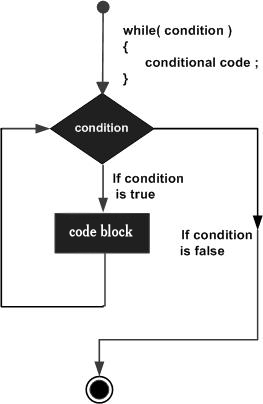
\includegraphics[scale=0.45]{while}
        \end{figure}
    \end{columns}
\end{frame}

\begin{frame}[fragile]
    \frametitle{The \texttt{while} Loop -- Syntax}
    \subsection{Syntax} % (fold)
    \label{sub:while_syntax}
    \begin{columns}
        \column{0.4\textwidth}
        \lstset{style=mystyle}
\begin{lstlisting}
while(test)
    {
       statement;
       statement;
       statement;
       statement;
    }
\end{lstlisting}
        \column{0.57\textwidth}
            \begin{itemize}
            \item Keyword \texttt{while} followed by a pair of parentheses that contain a test expression
            \item Although there is no initialization expression, the loop variable must be initialized before the loop begins
            \item The body of the loop, delimited by the left and right braces, is the code to be executed each time through the loop
            \item Similarly, the loop body must also contain some statement that keeps updating the value of the loop variable
            \end{itemize}
    \end{columns}
\end{frame}

\begin{frame} [fragile]
    \frametitle{The \texttt{while} Loop -- Solved Example 1}
    \subsection{Solved Examples} % (fold)
    \label{sub:while_solved_examples}
    \subsubsection{Solved Example 1} % (fold)
    \label{subsub:while_solved_example_1}
    \lstset{style=mystyle}
    \begin{lstlisting}
// demonstrates WHILE loop
#include <iostream>
using namespace std;
int main()
{
    int num, eoi = -1;
    cout << "Enter a number: ";
    cin >> num;

    while(num != eoi)
    {
        if(num % 2 == 0)
            cout << "The number is even.\n";
        else
            cout << "The number is odd.\n";
        cout << "Enter a number: ";
        cin >> num;
    }
    return 0;
}
\end{lstlisting}
\end{frame}

\begin{frame} [fragile]
    \frametitle{The \texttt{while} Loop -- Solved Example 2}
    \subsubsection{Solved Example 2} % (fold)
    \label{ssub:while_solved_example_2}
    \begin{columns}
        \column{0.67\textwidth}
        \lstset{style=mystyle}
\begin{lstlisting}
// sum using while loop (buggy)
#include <iostream>
using namespace std;

int main()
{
    int num = 0, sum = 0;
    while(num != -1)
    {
        cout << "Enter a number: ";
        cin >> num;

        sum = sum + num;
    }
    cout << "Sum = " << sum << endl;

    return 0;
}
\end{lstlisting}
        \column{0.3\textwidth}
            \begin{figure}
                \centering
                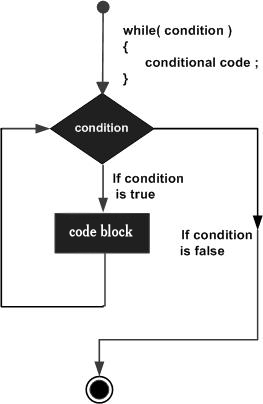
\includegraphics[scale=0.4]{while}
            \end{figure}
    \end{columns}
\end{frame}

\begin{frame} [fragile]
    \frametitle{The \texttt{while} Loop -- Solved Example 2}
    \begin{columns}
        \column{0.67\textwidth}
        \lstset{style=mystyle}
\begin{lstlisting}
// sum using while loop (fixed)
#include <iostream>
using namespace std;

int main()
{
    int num, sum = 0;
    cout << "Enter a number: ";
    cin >> num;

    while(num != -1)
    {
        sum = sum + num;

        cout << "Enter a number: ";
        cin >> num;
    }
    cout << "Sum = " << sum << endl;
    return 0;
}
\end{lstlisting}
        \column{0.3\textwidth}
            \begin{figure}
                \centering
                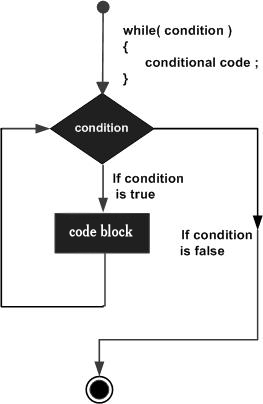
\includegraphics[scale=0.4]{while}
            \end{figure}
    \end{columns}
\end{frame}

\begin{frame} [fragile]
    \frametitle{Exercise}
    \subsection{Exercise} % (fold)
    \label{subsec:while_exercise}
    Write a calculator using \texttt{while} loop which keeps on getting a number and an operator as an input until `q' is entered as an operator. As soon as `q' is entered, the total result of the calculation is displayed and the execution of the program is stopped. \\ [0.2 in]
    Here goes a sample interaction with the program: \\
    \lstset{style=mystyle}
\begin{lstlisting}
Number: 5
Operator: +
Number: 5
Operator: *
Number: 3
Operator: -
Number: 2
Operator: /
Number: 2
Operator: q

Answer = 14
\end{lstlisting}
\end{frame}

\begin{frame}
    \frametitle{The \texttt{do} Loop}
    \section{The \texttt{do} Loop} % (fold)
    \label{sec:the_do_loop}
    \subsection{Importance} % (fold)
    \label{sub:importance_do}
    \begin{columns}
        \column{0.65\textwidth}
        \begin{itemize}
            \item In some situations, you want the test expression to be evaluated at the beginning of the loop
            \item But sometimes you want to guarantee that the loop is executed atleast once, no matter what the initial state of the test expression
            \item When such is the case, \texttt{do} loop should be used
        \end{itemize}
        \column{0.35\textwidth}
        \begin{figure}
            \centering
            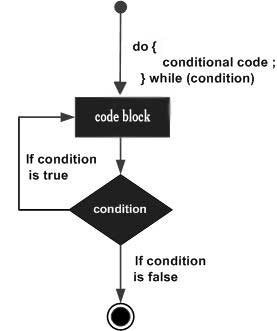
\includegraphics[scale=0.45]{do}
        \end{figure}
    \end{columns}
\end{frame}

\begin{frame}[fragile]
    \frametitle{The \texttt{do} Loop -- Syntax}
    \subsection{Syntax} % (fold)
    \label{sub:do_syntax}
    \begin{columns}
        \column{0.4\textwidth}
        \lstset{style=mystyle}
\begin{lstlisting}
do
    {
       statement;
       statement;
       statement;
       statement;
    }
while(test);
\end{lstlisting}
        \column{0.57\textwidth}
            \begin{itemize}
            \item Keyword \texttt{do} marks the beginning of the loop
            \item As with other loops, braces delimit the body of the loop
            \item Finally, a \texttt{while} statement provides the test expression and terminates the loop
            \end{itemize}
    \end{columns}
\end{frame}

\begin{frame} [fragile]
    \frametitle{The \texttt{do} Loop -- Solved Example}
    \subsection{Solved Example} % (fold)
    \label{sub:do_solved_example}
    \lstset{style=mystyle}
    \begin{lstlisting}
#include <iostream>
using namespace std;
int main()
{
    int dividend, divisor;
    char ch;
    do
        {
            cout << "Enter dividend: ";
            cin >> dividend;
            cout << "Enter divisor: ";
            cin >> divisor;
            cout << "Quotient is " << dividend / divisor;
            cout << ", remainder is " << dividend % divisor;
            cout << "\nDo another? (y/n): ";
            cin >> ch;
        }
    while(ch != 'n');
return 0;
}
\end{lstlisting}
\end{frame}

\begin{frame} [fragile]
    \frametitle{Exercise}
    \subsection{Exercise} % (fold)
    \label{subsec:do_exercise}
    Write a program using \texttt{do} loop that repeatedly asks for a number and calculates its factorial until the user enters 0, at which point it terminates. \\ [0.2 in]
    Here goes a sample interaction with the program: \\
    \lstset{style=mystyle}
\begin{lstlisting}
Enter a number: 7
The factorial of the number is: 5040
Enter a number: 6
The factorial of the number is: 720
Enter a number: 5
The factorial of the number is: 120
Enter a number: 0
The factorial of the number is: 1
\end{lstlisting}
\end{frame}

\begin{frame}
    \frametitle{When to Use Which Loop?}
    \section{When to Use Which Loop?} % (fold)
    \label{sec:which}
    \begin{itemize}
        \item Which loop type to use is more a matter of style than of hard-and-fast rules
        \item The \texttt{for} loop is appropriate when you know in advance how many times the loop will be executed
        \item The \texttt{while} and \texttt{do} loops are used when you don't know the number of times a loop will be executed
        \begin{itemize}
            \item The \texttt{while} loop when you may not want to execute the loop body even once
            \item The \texttt{do} loop when you're sure you want to execute the loop body at least once
        \end{itemize}
    \end{itemize}
\end{frame}
\end{document}